\documentclass[10pt,a4paper,twoside]{article}
\usepackage{pstricks}
\usepackage{fancybox}
\usepackage{amsfonts}
% \usepackage{minitoc}
% \setcounter{minitocdepth}{2}
\usepackage[bookmarks=true, 
            bookmarksnumbered=true, 
            bookmarksopen=false, 
            plainpages=false,
            pdfpagelabels,
            colorlinks, 
            citecolor=red,
            linkcolor=blue]{hyperref}
\usepackage{ifthen}
\usepackage{graphicx}
\newtheorem{theorem}{Theorem}
\newtheorem{corollary}{Corollary}
\usepackage{listings}
\usepackage{algorithm2e}

%\newboolean{mtc}
%\setboolean{mtc}{true}

\pdfoutput=1
\relax
\pdfcompresslevel=0             %-- 0 = none, 9 = best
\pdfinfo{                       %-- Info dictionary of PDF output  /Author (Alfredo Buttari)
  /Title (Parallel Sparse BLAS  Extensions)
  /Subject (Parallel Sparse Basic Linear Algebra Subroutines)
  /Keywords (Computer Science Linear Algebra Fluid Dynamics Parallel Linux MPI PSBLAS Iterative Solvers Preconditioners)
  /Creator (pdfLaTeX)
  /Producer ($Id: userguide.tex 7725 2014-03-21 08:58:20Z sfilippo $)
}
\pdfcatalog{          %-- Catalog dictionary of PDF output.
  /URI (http://ce.uniroma2.it/psblas)
} 

\newcounter{subroutine}[subsection]
\newcounter{example}[subroutine]
\makeatletter
\def\subroutine{\@ifstar{\@subroutine}{\clearpage\@subroutine}}%
\def\@subroutine#1#2{%
\stepcounter{subroutine}%
      \section*{\flushleft #1---#2 \endflushleft}%
      \addcontentsline{toc}{subsection}{#1}%
      \markright{#1}}%
\newcommand{\subsubroutine}[2]{%
\stepcounter{subroutine}%
      \subsubsection*{\flushleft #1---#2 \endflushleft}%
      \addcontentsline{toc}{subsubsection}{#1}%
      \markright{#1}}%

\newcommand{\subsubsubroutine}[2]{%
\stepcounter{subroutine}%
      \subsubsection*{\flushleft #1---#2 \endflushleft}%
      \addcontentsline{toc}{paragraph}{#1}%
      \markright{#1}}%

\newcommand{\examplename}{Example}
\newcommand{\syntaxname}{Syntax}
\def\syntax{\@ifstar{\@ssyntax}{\@syntax}}%
\def\@syntax{\nobreak\section*{\syntaxname}%
     \@ssyntax}%
\def\@ssyntax#1#2{%
  \nobreak
   \setbox\@tempboxa\hbox{#1\ {\em $($#2$)$}}%
   \ifdim \wd\@tempboxa >\hsize
        \setbox\@tempboxa\hbox{\em $($#2$)$}
	\ifdim\wd\@tempboxa >\hsize
          \flushright#1\ \em$($#2$)$\endflushright%
	\else
         \hbox to\hsize{#1\hfil}%
         \hbox to\hsize{\hfil\box\@tempboxa}%
        \fi
     \else
       \hbox to\hsize{\hfil\box\@tempboxa\hfil}%
   \fi\par\vskip\baselineskip}
\makeatother
\newcommand{\example}{\stepcounter{example}%
\section*{\examplename~\theexample}}

\newcommand{\precdata}{\hyperlink{precdata}{{\tt psb\_prec\_type}}}
\newcommand{\descdata}{\hyperlink{descdata}{{\tt psb\_desc\_type}}}
\newcommand{\spdata}{\hyperlink{spdata}{{\tt psb\_Tspmat\_type}}}
\newcommand{\vdata}{\hyperlink{vdata}{{\tt psb\_T\_vect\_type}}}
\newcommand{\spbasedata}{\hypertarget{spbasedata}{{\tt psb\_T\_base\_sparse\_mat}}}
\newcommand{\vbasedata}{\hypertarget{vbasedata}{{\tt psb\_T\_base\_vect\_type}}}

\begin{document}

\pdfbookmark{PSBLAS-Extentions v1.0}{title}
\lstset{language=Fortran}
\newlength{\centeroffset}
\setlength{\centeroffset}{-0.5\oddsidemargin}
\addtolength{\centeroffset}{0.5\evensidemargin}
%\addtolength{\textwidth}{-\centeroffset}
\thispagestyle{empty}
\vspace*{\stretch{1}}
\noindent\hspace*{\centeroffset}\makebox[0pt][l]{\begin{minipage}{\textwidth}
\flushright
{\Huge\bfseries PSBLAS-Extensions  1.0
}
\noindent\rule[-1ex]{\textwidth}{5pt}\\[2.5ex]
\hfill\emph{\Large A reference guide for the Parallel Sparse BLAS library}
\end{minipage}}

\vspace{\stretch{1}}
\noindent\hspace*{\centeroffset}\makebox[0pt][l]{\begin{minipage}{\textwidth}
\flushright
{\bfseries 
by Salvatore Filippone}\\ 
University of Rome ``Tor Vergata''.\\[3ex]
March 25, 2015.
\end{minipage}}

%\addtolength{\textwidth}{\centeroffset}
\vspace{\stretch{2}}
\setcounter{tocdepth}{4}

\cleardoublepage
\begingroup
  \renewcommand*{\thepage}{toc}
  \pagenumbering{roman}   % Roman numbering
  \setcounter{page}{1}    % Abstract start on page ii
  \tableofcontents
\endgroup  

\cleardoublepage

\pagenumbering{arabic}  % Arabic numbering
\setcounter{page}{1}    % Chapters start on page 1

\section{Introduction}\label{sec:intro}

The PSBLAS-EXT  library contains a set of extensions to the base
library. The extensions provide additional storage formats beyond the
 ones already contained in the base library, as well as interfaces to
 two external libraries:
\begin{itemize}
\item SPGPU \url{https://code.google.com/p/spgpu/}, for computations on
  NVIDIA GPUs;
\item LIBRSB \url{http://sourceforge.net/projects/librsb/}, for
  computations on multicore parallel machines. 
\end{itemize}
The infrastructure laid out in the base library to allow for these
extensions is detailed in the references~\cite{CaFiRo:14,Sparse03}. 


\subsection{Application structure}
\label{sec:appstruct}
A sample application using the PSBLAS extensions will contain the
following steps:
\begin{itemize}
\item \verb|USE| the appropriat modules (\verb|psb_ext_mod|,
  \verb|psb_gpu_mod|);
\item Declare a \emph{mold} variable of the necessary type
  (e.g. \verb|psb_d_ell_sparse_mat|, \verb|psb_d_hlg_sparse_mat|,
  \verb|psb_d_vect_gpu|);
\item Pass the mold variable to the base library interface where
  needed to ensure the appropriate dynamic type.
\end{itemize}
Suppose you want to use the GPU-enabled ELLPACK data structure; you
would use a piece of code like this (and don't forget, you need
GPU-side vectors along with the matrices):
\lstset{language=Fortran}
\begin{lstlisting}
program my_gpu_test
  use psb_base_mod
  use psb_util_mod 
  use psb_ext_mod
  use psb_gpu_mod
  type(psb_dspmat_type) :: a, agpu
  type(psb_d_vect_type) :: x, xg, bg

  real(psb_dpk_), allocatable :: xtmp(:)
  type(psb_d_vect_gpu)       :: vmold
  type(psb_d_elg_sparse_mat) :: aelg

  ......  

  ! My own home-grown matrix generator
  call gen_matrix(ictxt,idim,desc_a,a,x,info)
  
  call a%cscnv(agpu,info,mold=aelg)
  xtmp = x%get_vect() 
  call xg%bld(xtmp,mold=vmold)
  call bg%bld(size(xtmp),mold=vmold)
  
  ! Do sparse MV
  call psb_spmm(done,agpu,xg,dzero,bg,desc_a,info)
\end{lstlisting}
A full example of this strategy can be seen in the
\verb|test/ext/kernel| subdirectory, where we provide a sample program
to test the speed of the sparse matrix-vector product with the various
data structures included in the library. 





%%% Local Variables: 
%%% mode: latex
%%% TeX-master: "userguide"
%%% End: 

\section{Data Structures}
\label{sec:datastruct}
%\ifthenelse{\boolean{mtc}}{\minitoc}{}

Access to the facilities provided by \verb|psblas-ext| is mainly
through the data types that are provided within. 
The data classes are derived from the base  classes in PSBLAS, through 
the Fortran~2003 mechanism of \emph{type extension}~\cite{MRC:11}.  

The data classes are divided between the general purpose CPU
extensions, the GPU interfaces and the RSB interfaces.

In the description we will make use of the notation introduced in
Table~\ref{tab:notation}. 

\begin{table}[ht]
\caption{Notation for parameters describing a sparse matrix}
\begin{center}
{\footnotesize
\begin{tabular}{ll}
\hline
Name & Description \\
\hline
M		& Number of rows in matrix		 \\
N		& Number of columns in matrix		 \\
NZ              & Number of nonzeros in matrix   \\
AVGNZR          & Average number of nonzeros per row  \\
MAXNZR          & Maximum number of nonzeros per row  \\
NDIAG           & Numero of nonzero diagonals\\
AS	        & Coefficients 	array		 \\
IA	        & Row indices array			 \\
JA	        & Column  indices array			 \\
IRP	        & Row start pointers array			 \\
JCP	        & Column start pointers array			 \\
NZR 	        & Number of nonzeros per row array \\
OFFSET          & Offset for diagonals			 \\
\hline
\end{tabular}
}
\end{center}
\label{tab:notation}
\end{table}

\begin{figure}[ht]
	\centering
%		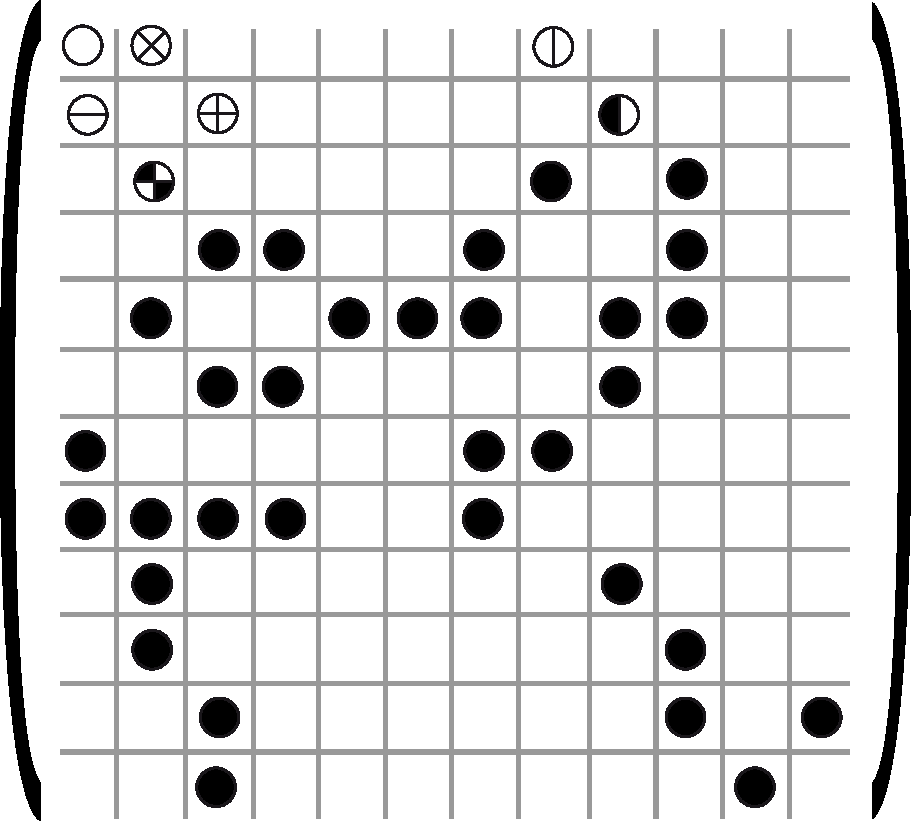
\includegraphics[width=5.2cm]{images/mat.eps}
		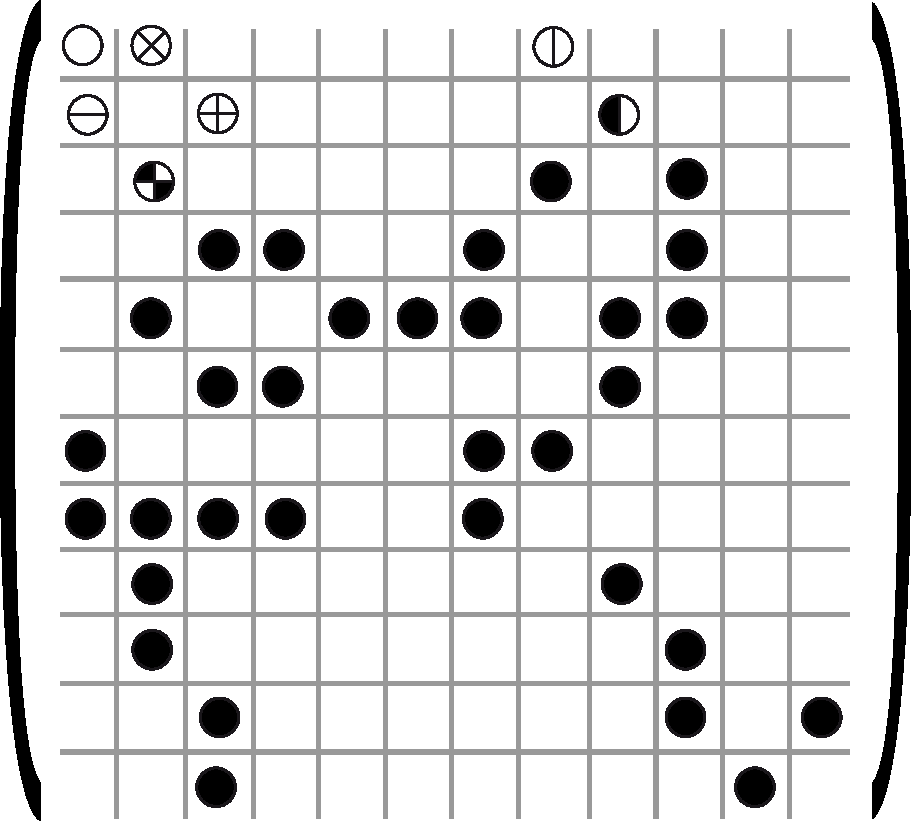
\includegraphics[width=5.2cm]{images/mat.pdf}
	\caption{Example of sparse matrix}
	\label{fig:dense}
\end{figure} 

\subsection{CPU-class extensions}


\subsubsection*{ELLPACK}

The ELLPACK/ITPACK format (shown in Figure~\ref{fig:ell}) 
comprises  two 2-dimensional arrays \verb|AS| and
\verb|JA|  with \verb|M| rows and \verb|MAXNZR| columns, where
\verb|MAXNZR| is the maximum
number of nonzeros in any row~\cite{ELLPACK}. 
Each row of the arrays \verb|AS| and \verb|JA| contains the
coefficients and column indices; rows shorter than
\verb|MAXNZR| are padded with zero coefficients and appropriate column
indices, e.g. the last valid one found in the same row.

\begin{figure}[ht]
	\centering
%		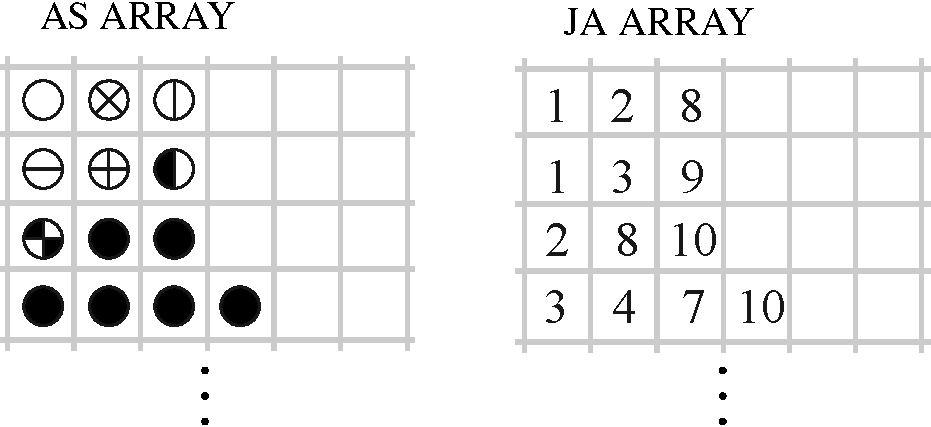
\includegraphics[width=8.2cm]{images/ell.eps}
		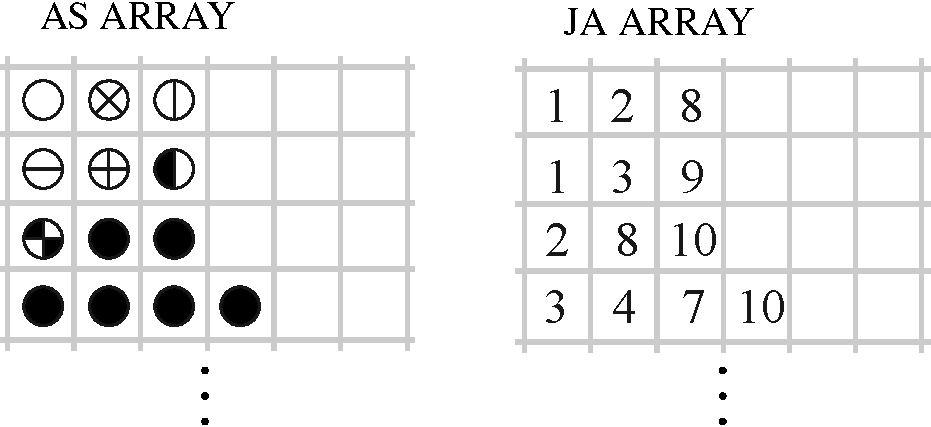
\includegraphics[width=8.2cm]{images/ell.pdf}
	\caption{ELLPACK compression of matrix in Figure~\ref{fig:dense}}
	\label{fig:ell}
\end{figure} 


\begin{algorithm}
\lstset{language=Fortran}
\small
  \begin{lstlisting}
    do i=1,n
      t=0
      do j=1,maxnzr
        t = t +  as(i,j)*x(ja(i,j))
      end do
      y(i) = t
    end do
  \end{lstlisting}
  \caption{\label{alg:ell} Matrix-Vector product in ELL format}
\end{algorithm}
The matrix-vector product $y=Ax$ can be computed with the code shown in
Alg.~\ref{alg:ell}; it costs  one  memory write per outer iteration, 
plus three memory reads  and two floating-point operations per inner
iteration.   

Unless all rows have exactly the same number of nonzeros, some of the
coefficients in the \verb|AS| array will be zeros; therefore this
data structure will have  an overhead both in terms of memory space
and redundant operations (multiplications by zero).  The overhead can
be acceptable if: 
\begin{enumerate}
\item The maximum number of nonzeros per row is not much larger than
  the    average;
\item The regularity of the data structure allows for faster  code,
  e.g. by allowing vectorization, thereby offsetting the additional
  storage requirements.  
\end{enumerate}
In the extreme case where the input matrix has one full row, the
ELLPACK structure would require more memory than the normal 2D array
storage. The ELLPACK storage format was very popular in the vector
computing days; in modern CPUs it is not quite as popular, but it
is  the basis for many GPU formats. 

The relevant data type is \verb|psb_T_ell_sparse_mat|:
\begin{minted}[breaklines=true,bgcolor=bg,fontsize=\small]{fortran}
  type, extends(psb_d_base_sparse_mat) :: psb_d_ell_sparse_mat
    !
    ! ITPACK/ELL format, extended.
    !     
    
    integer(psb_ipk_), allocatable :: irn(:), ja(:,:), idiag(:)
    real(psb_dpk_), allocatable :: val(:,:)

  contains
    ....
  end type psb_d_ell_sparse_mat
\end{minted}


\subsubsection*{Hacked ELLPACK}

The \textit{hacked ELLPACK} (\textbf{HLL}) format 
alleviates the main problem of the ELLPACK format, that is, 
the  amount of  memory required by  padding for  sparse matrices in
which the maximum row length is  larger than the average.

The number of  elements  allocated to padding is $[(m*maxNR) -
(m*avgNR) = m*(maxNR-avgNR)]$ 
for both \verb|AS|  and \verb|JA| arrays,
where $m$ is equal to the number of rows of the matrix, $maxNR$ is the
maximum number of nonzero elements 
in every row and $avgNR$ is the average number of nonzeros. 
Therefore a single densely populated row can seriously affect the
total size of the allocation. 

To limit this effect, in the HLL format  we break the original matrix
into equally sized groups of rows (called \textit{hacks}), and then store
these groups as independent matrices in ELLPACK format. 
The groups can be arranged selecting rows in an arbitrarily manner;
indeed, if the rows are sorted by decreasing number of nonzeros we
obtain essentially the JAgged Diagonals format. 
If the rows are not in the original order, then an   additional vector
\textit{rIdx} is required, storing the actual row index  for each row
in the data structure.

The multiple ELLPACK-like buffers are stacked together inside a
single, one dimensional array; 
an additional  vector \textit{hackOffsets} is provided to keep track
of the individual submatrices.
All hacks have the same number of rows  \textit{hackSize}; hence, 
the \textit{hackOffsets} vector is  an array of
$(m/hackSize)+1$ elements, each one pointing  to the first index of a
submatrix inside the stacked \textit{cM}/\textit{rP} buffers, plus an
additional element pointing past the end of the last block, where the
next one would begin. 
We thus have the property that  
the elements of the $k$-th \textit{hack} are stored between \verb|hackOffsets[k]| and
\verb|hackOffsets[k+1]|, similarly to what happens in the CSR format. 

\begin{figure}[ht]
	\centering
%		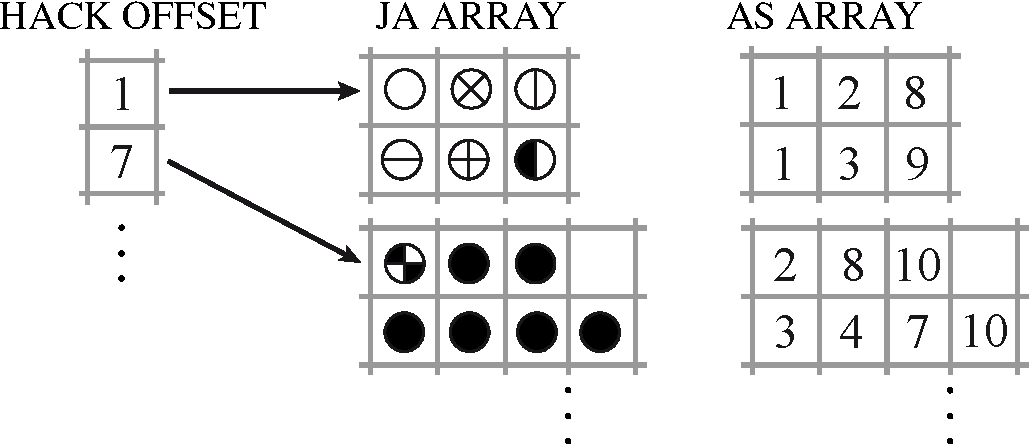
\includegraphics[width=8.2cm]{../images/hll.eps}
	 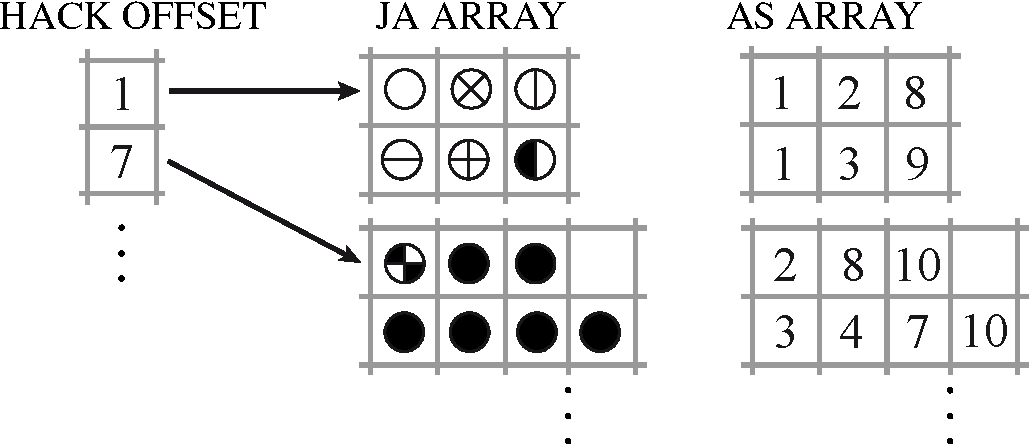
\includegraphics[width=.72\textwidth]{../images/hll.pdf}
	\caption{Hacked ELLPACK compression of matrix in Figure~\ref{fig:dense}}
	\label{fig:hll}
\end{figure} 

With this data structure a very long row only affects one hack, and
therefore the additional memory is limited to the hack in which the
row appears.

The relevant data type is \verb|psb_T_hll_sparse_mat|:
\begin{minted}[breaklines=true,bgcolor=bg,fontsize=\small]{fortran}
  type, extends(psb_d_base_sparse_mat) :: psb_d_hll_sparse_mat
    !
    ! HLL format. (Hacked ELL) 
    !     
    integer(psb_ipk_) :: hksz
    integer(psb_ipk_), allocatable :: irn(:), ja(:), idiag(:), hkoffs(:)
    real(psb_dpk_), allocatable :: val(:)

  contains
   ....
  end type
\end{minted}

\subsubsection*{Diagonal storage}


The DIAgonal (DIA) format (shown in Figure~\ref{fig:dia}) 
has   a 2-dimensional array \verb|AS| containing in each column the
coefficients along a  diagonal of the matrix, and an integer array
\verb|OFFSET|  that determines  where each diagonal starts. The
diagonals in \verb|AS| are padded with zeros as necessary. 

The code to compute the matrix-vector product $y=Ax$ is shown in Alg.~\ref{alg:dia};
it costs one  memory read per outer iteration, 
plus three memory reads, one memory write  and two floating-point
operations per inner iteration. The accesses to  \verb|AS| and
\verb|x| are in strict sequential order,  therefore no indirect
addressing is required.  

\begin{figure}[ht]
	\centering
%		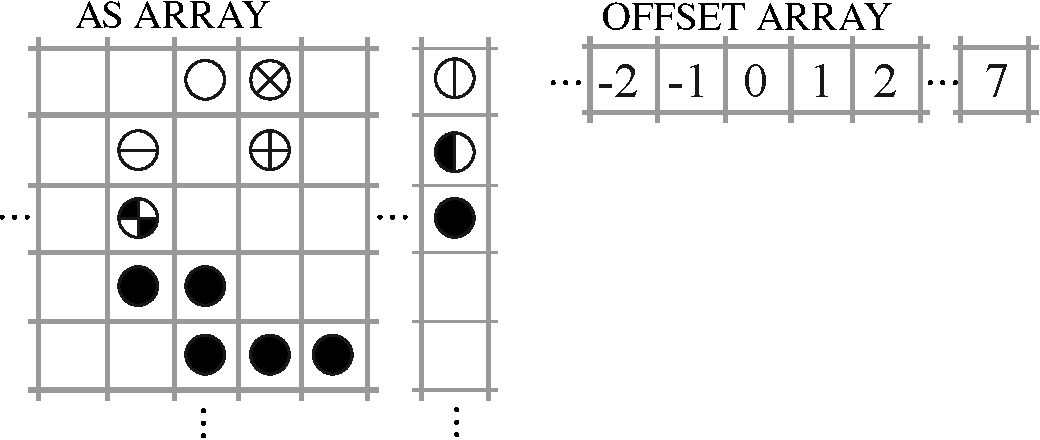
\includegraphics[width=8.2cm]{images/dia.eps}
		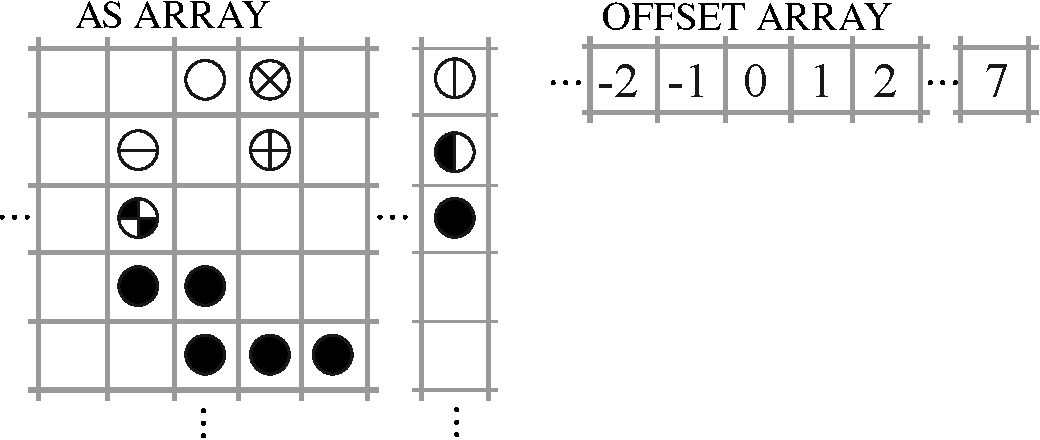
\includegraphics[width=.72\textwidth]{images/dia.pdf}
	\caption{DIA compression of matrix in Figure~\ref{fig:dense}}
	\label{fig:dia}
\end{figure} 


\begin{algorithm}
\begin{minted}[breaklines=true,bgcolor=bg,fontsize=\small]{fortran}
    do j=1,ndiag
      if (offset(j) > 0) then 
        ir1 = 1; ir2 = m - offset(j);
      else
        ir1 = 1 - offset(j); ir2 = m;
      end if
      do i=ir1,ir2
        y(i) = y(i) + alpha*as(i,j)*x(i+offset(j))
      end do
    end do
\end{minted}
  \caption{\label{alg:dia} Matrix-Vector product in DIA format}
\end{algorithm}


The relevant data type is \verb|psb_T_dia_sparse_mat|:
\begin{minted}[breaklines=true,bgcolor=bg,fontsize=\small]{fortran}
  type, extends(psb_d_base_sparse_mat) :: psb_d_dia_sparse_mat
    !
    ! DIA format, extended.
    !     
    
    integer(psb_ipk_), allocatable :: offset(:)
    integer(psb_ipk_) :: nzeros
    real(psb_dpk_), allocatable :: data(:,:)

  end type
\end{minted}



\subsubsection*{Hacked DIA}

Storage by DIAgonals is an attractive option for matrices whose
coefficients are located on a small set of diagonals, since they do
away with storing explicitly the indices and therefore reduce
significantly memory traffic. However, having a few coefficients
outside of the main set of diagonals may  significantly increase the
amount of needed padding; moreover, while the DIA code is easily
vectorized, it does not necessarily make optimal use of the memory
hierarchy. While processing each diagonal we are updating entries in
the output vector \verb|y|, which is then accessed multiple times; if 
the vector \verb|y| is too large to remain in the cache memory, the
associated cache miss penalty is paid multiple times. 

The \textit{hacked DIA} (\textbf{HDIA}) format was designed to contain
the amount of padding, by  breaking  the original matrix
into equally sized groups of rows (\textit{hacks}), and then storing
these groups as independent matrices in DIA format. This approach is
similar to that of HLL, and requires using an offset vector for each
submatrix. Again, similarly to HLL, the various submatrices are
stacked inside a linear array to improve memory management. The fact
that the matrix is accessed in slices helps in reducing cache misses,
especially regarding accesses to the %output 
vector \verb|y|.  


An additional vector \textit{hackOffsets} is provided to complete
the matrix format; given  that \textit{hackSize} is the number of rows of each hack,
the \textit{hackOffsets} vector is made by an array of
$(m/hackSize)+1$ elements,  pointing to the first diagonal offset of a
submatrix inside the stacked \textit{offsets} buffers, plus an
additional element equal to the number of nonzero diagonals in the whole matrix. 
We thus have the property that  
the number of diagonals of the $k$-th \textit{hack} is given by
\textit{hackOffsets[k+1] - hackOffsets[k]}.  

\begin{figure}[ht]
	\centering
%		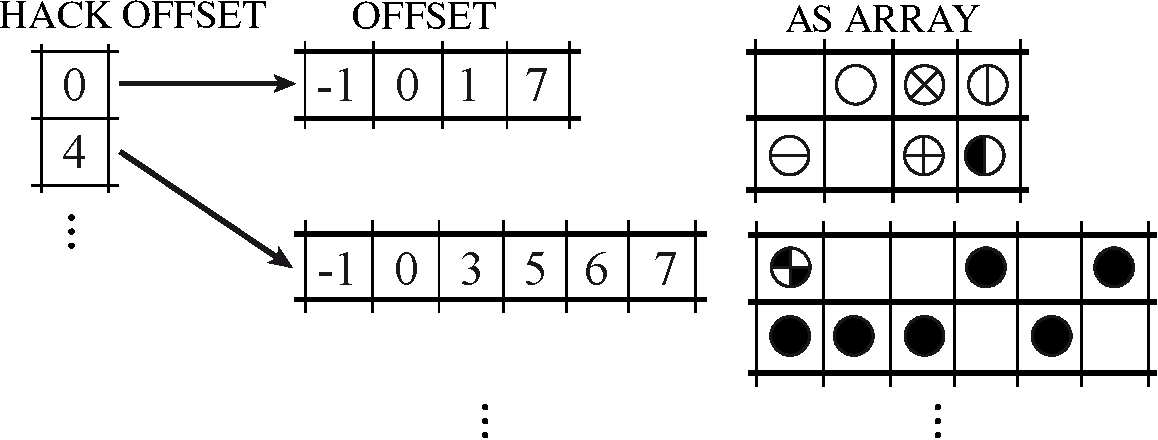
\includegraphics[width=8.2cm]{../images/hdia.eps}
		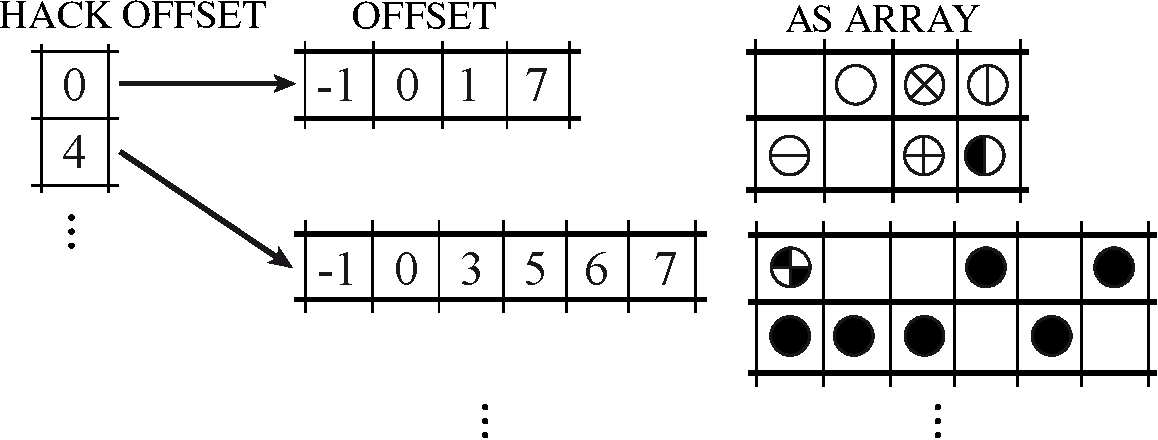
\includegraphics[width=.72\textwidth]{../images/hdia.pdf}
	\caption{Hacked DIA compression of matrix in Figure~\ref{fig:dense}}
	\label{fig:hdia}
\end{figure} 

The relevant data type is \verb|psb_T_hdia_sparse_mat|:
\begin{minted}[breaklines=true,bgcolor=bg,fontsize=\small]{fortran}
  type pm
     real(psb_dpk_), allocatable  :: data(:,:)
  end type pm

  type po
     integer(psb_ipk_), allocatable  :: off(:)
  end type po

  type, extends(psb_d_base_sparse_mat) :: psb_d_hdia_sparse_mat
    !
    ! HDIA format, extended.
    !
    
    type(pm), allocatable :: hdia(:)
    type(po), allocatable :: offset(:)
    integer(psb_ipk_) :: nblocks, nzeros
    integer(psb_ipk_) :: hack = 64
    integer(psb_long_int_k_) :: dim=0

  contains
   ....
  end type
\end{minted}



\subsection{GPU-class extensions}

For computing on the GPU we define a dual memorization strategy in
which each variable on the CPU (``host'') side has a GPU (``device'')
side. When a GPU-type variable is initialized, the data contained is
(usually) the same on both sides. Each operator invoked on the
variable may change the data so that only the host side or the device
side are up-to-date. 

Keeping track of the updates to data in the variables  is essential: we want
to perform most  computations on the GPU, but we cannot afford the time
needed to move data between the host  memory and the device memory
because the bandwidth of the interconnection bus would become the main
bottleneck of the computation. Thus, each and every computational
routine in the library is built according to the following principles: 
\begin{itemize}
\item If the data type being handled is {GPU}-enabled, make sure that
  its device copy is up to date, perform any arithmetic operation on
  the {GPU}, and if the data has been altered as a result, mark
  the main-memory copy as outdated.
\item The main-memory copy is never updated unless this is requested
  by the user either 
\begin{description}
\item[explicitly] by invoking a synchronization method;
\item[implicitly] by invoking a method that involves other data items
  that are not {GPU}-enabled, e.g., by assignment ov a vector to a
  normal array. 
\end{description}
\end{itemize}
In this way, data items are put on the {GPU} memory ``on demand'' and
remain there as long as ``normal'' computations are carried out. 
As an example, the following call to a matrix-vector product
\begin{minted}[breaklines=true,bgcolor=bg,fontsize=\small]{fortran}
    call psb_spmm(alpha,a,x,beta,y,desc_a,info)
\end{minted}
will transparently and automatically be performed on the {GPU} whenever
all three data inputs \fortinline|a|, \fortinline|x|  and
\fortinline|y| are {GPU}-enabled. If a program makes many such calls
sequentially, then 
\begin{itemize}
\item The first kernel invocation will find the data in main memory,
  and will copy it to the {GPU} memory, thus incurring a significant
  overhead; the result is however \emph{not} copied back, and
  therefore:
\item Subsequent kernel invocations involving the same vector will
  find the data on the {GPU} side so that they will run at full
  speed.
\end{itemize}
For all invocations after the first the only data that will have to be
transferred to/from the main memory will be the scalars \fortinline|alpha|
and \fortinline|beta|, and the return code \fortinline|info|.  

\begin{description}
\item[Vectors:] The data type \fortinline|psb_T_vect_gpu| provides a
  GPU-enabled extension of the inner type \fortinline|psb_T_base_vect_type|,
  and must be used together with the other inner matrix type to make
  full use of the GPU computational capabilities;
\item[CSR:] The data type \fortinline|psb_T_csrg_sparse_mat| provides an
  interface to the GPU version of CSR available in the NVIDIA CuSPARSE
  library;
\item[HYB:] The data type \fortinline|psb_T_hybg_sparse_mat| provides an
  interface to the HYB GPU storage  available in the NVIDIA CuSPARSE
  library. The internal structure is opaque, hence the host side is
  just CSR; the HYB data format is only available up to CUDA version
  10. 
\item[ELL:] The data type \fortinline|psb_T_elg_sparse_mat| provides an
  interface to the  ELLPACK implementation from SPGPU;

\item[HLL:] The data type \fortinline|psb_T_hlg_sparse_mat| provides an
  interface to the  Hacked ELLPACK implementation from SPGPU;
\item[HDIA:] The data type \fortinline|psb_T_hdiag_sparse_mat| provides an
  interface to the  Hacked DIAgonals implementation from SPGPU;
\end{description}


%%% Local Variables: 
%%% mode: latex
%%% TeX-master: "userguide"
%%% End: 

%\include{psbrout}
%\include{commrout}
%\include{toolsrout}

\section{GPU Environment Routines}
\label{sec:gpuenv}

\subsection*{psb\_gpu\_init --- Initializes PSBLAS-GPU
  environment}
\addcontentsline{toc}{subsection}{psb\_gpu\_init}

\begin{minted}[breaklines=true]{fortran}
call psb_gpu_init(ctxt [, device])
\end{minted}

This subroutine initializes the PSBLAS-GPU  environment. 
\begin{description}
\item[Type:] Synchronous.
\item[\bf  On Entry ]
\item[device] ID of GPU device to attach to.\\
Scope: {\bf local}.\\
Type: {\bf optional}.\\
Intent: {\bf in}.\\
Specified as: an integer value. \
Default: use \fortinline|mod(iam,ngpu)| where \fortinline|iam| is the calling
process index and \fortinline|ngpu| is the total number of GPU devices
available on the current node. 
\end{description}


{\par\noindent\large\bfseries Notes}
\begin{enumerate}
\item A call to this routine must precede any other PSBLAS-GPU call. 
\end{enumerate}

\subsection*{psb\_gpu\_exit --- Exit from  PSBLAS-GPU
  environment}
\addcontentsline{toc}{subsection}{psb\_gpu\_exit}

\begin{minted}[breaklines=true]{fortran}
call psb_gpu_exit(ctxt)
\end{minted}

This subroutine exits from the  PSBLAS GPU context.
\begin{description}
\item[Type:] Synchronous.
\item[\bf  On Entry ]
\item[ctxt] the communication context identifying the virtual
  parallel machine.\\
Scope: {\bf global}.\\
Type: {\bf required}.\\
Intent: {\bf in}.\\
Specified as: an integer variable.
\end{description}




\subsection*{psb\_gpu\_DeviceSync ---  Synchronize GPU device}
\addcontentsline{toc}{subsection}{psb\_gpu\_DeviceSync}

\begin{minted}[breaklines=true]{fortran}
call psb_gpu_DeviceSync()
\end{minted}

This subroutine ensures that all previosly invoked kernels, i.e. all
invocation of GPU-side code, have completed.


\subsection*{psb\_gpu\_getDeviceCount }
\addcontentsline{toc}{subsection}{psb\_gpu\_getDeviceCount}

\begin{minted}[breaklines=true]{fortran}
ngpus =  psb_gpu_getDeviceCount()
\end{minted}

Get number of devices available on current computing node. 

\subsection*{psb\_gpu\_getDevice }
\addcontentsline{toc}{subsection}{psb\_gpu\_getDevice}

\begin{minted}[breaklines=true]{fortran}
ngpus =  psb_gpu_getDevice()
\end{minted}

Get  device in use by current process. 

\subsection*{psb\_gpu\_setDevice }
\addcontentsline{toc}{subsection}{psb\_gpu\_setDevice}

\begin{minted}[breaklines=true]{fortran}
info = psb_gpu_setDevice(dev)
\end{minted}

Set  device to be used  by current process. 

\subsection*{psb\_gpu\_DeviceHasUVA }
\addcontentsline{toc}{subsection}{psb\_gpu\_DeviceHasUVA}

\begin{minted}[breaklines=true]{fortran}
hasUva = psb_gpu_DeviceHasUVA()
\end{minted}

Returns true if device currently in use supports UVA (Unified Virtual Addressing).

\subsection*{psb\_gpu\_WarpSize }
\addcontentsline{toc}{subsection}{psb\_gpu\_WarpSize}

\begin{minted}[breaklines=true]{fortran}
nw = psb_gpu_WarpSize()
\end{minted}

Returns the warp size.


\subsection*{psb\_gpu\_MultiProcessors }
\addcontentsline{toc}{subsection}{psb\_gpu\_MultiProcessors}

\begin{minted}[breaklines=true]{fortran}
nmp = psb_gpu_MultiProcessors()
\end{minted}

Returns the number of multiprocessors in the GPU device.

\subsection*{psb\_gpu\_MaxThreadsPerMP }
\addcontentsline{toc}{subsection}{psb\_gpu\_MaxThreadsPerMP}

\begin{minted}[breaklines=true]{fortran}
nt = psb_gpu_MaxThreadsPerMP()
\end{minted}

Returns the maximum number of threads per multiprocessor. 


\subsection*{psb\_gpu\_MaxRegistersPerBlock }
\addcontentsline{toc}{subsection}{psb\_gpu\_MaxRegisterPerBlock}

\begin{minted}[breaklines=true]{fortran}
nr = psb_gpu_MaxRegistersPerBlock()
\end{minted}

Returns the maximum number of register per thread block. 


\subsection*{psb\_gpu\_MemoryClockRate }
\addcontentsline{toc}{subsection}{psb\_gpu\_MemoryClockRate}

\begin{minted}[breaklines=true]{fortran}
cl = psb_gpu_MemoryClockRate()
\end{minted}

Returns the memory clock rate in KHz, as an integer. 

\subsection*{psb\_gpu\_MemoryBusWidth }
\addcontentsline{toc}{subsection}{psb\_gpu\_MemoryBusWidth}

\begin{minted}[breaklines=true]{fortran}
nb = psb_gpu_MemoryBusWidth()
\end{minted}

Returns the memory bus width in bits.

\subsection*{psb\_gpu\_MemoryPeakBandwidth }
\addcontentsline{toc}{subsection}{psb\_gpu\_MemoryPeakBandwidth}

\begin{minted}[breaklines=true]{fortran}
bw = psb_gpu_MemoryPeakBandwidth()
\end{minted}

Returns the memory peak bandwidth in MB/s (real double precision).




%\include{error}
%\include{util}
%\include{precs}
%\include{methods}

\cleardoublepage

\begin{thebibliography}{99}
\bibitem{OurTechRep}
D.~Barbieri, V.~Cardellini, A.~Fanfarillo, S.~Filippone, Three storage formats
  for sparse matrices on {GPGPUs}, Tech. Rep. DICII RR-15.6, Universit\`a di
  Roma Tor Vergata (February 2015).

\bibitem{CaFiRo:2014}
{ Cardellini, V.}, { Filippone, S.}, { and} { Rouson, D.} 2014,
 Design patterns for sparse-matrix computations on hybrid {CPU/GPU}
  platforms,
{\em Scientific Programming\/}~{\em 22,\/}~1, 1--19.

\bibitem{PSBLAS}
S.~Filippone and M.~Colajanni, 
{\em PSBLAS: A Library for Parallel Linear Algebra
Computation on Sparse Matrices},
\newblock
ACM Transactions on Mathematical Software, 26(4), pp.~527--550, 2000.
%
\bibitem{Sparse03}
S.~Filippone and A.~Buttari, 
{\em Object-Oriented Techniques for Sparse Matrix Computations in Fortran 2003},
\newblock
ACM Transactions on Mathematical Software, 38(4), 2012.
%
\bibitem{DesignPatterns}
{ Gamma, E.}, { Helm, R.}, { Johnson, R.}, { and} { Vlissides,
  J.} 1995.
 {\em Design Patterns: Elements of Reusable Object-Oriented Software}.
 Addison-Wesley.

%
\bibitem{MRC:11}
{Metcalf, M., Reid, J. and Cohen, M.}
{\em Modern Fortran  explained.}
{Oxford University Press}, 2011.
%
\end{thebibliography}


\end{document}
%%% Local Variables: 
%%% mode: latex
%%% TeX-master: 'userguide'
%%% End: 
